%%%%%%%%%%%%%%%%%%%%%%%%%%%%%%%%%%%%%%%%%
% Beamer Presentation
% LaTeX Template
% Version 1.0 (10/11/12)
%
% This template has been downloaded from:
% http://www.LaTeXTemplates.com
%
% License:
% CC BY-NC-SA 3.0 (http://creativecommons.org/licenses/by-nc-sa/3.0/)
%
%%%%%%%%%%%%%%%%%%%%%%%%%%%%%%%%%%%%%%%%%

%----------------------------------------------------------------------------------------
%	PACKAGES AND THEMES
%----------------------------------------------------------------------------------------

\documentclass{beamer}

\mode<presentation> {

% The Beamer class comes with a number of default slide themes
% which change the colors and layouts of slides. Below this is a list
% of all the themes, uncomment each in turn to see what they look like.

%\usetheme{default}
%\usetheme{AnnArbor}
%\usetheme{Antibes}
%\usetheme{Bergen}
%\usetheme{Berkeley}
%\usetheme{Berlin}
%\usetheme{Boadilla}
%\usetheme{CambridgeUS}
%\usetheme{Copenhagen}
%\usetheme{Darmstadt}
%\usetheme{Dresden}
%\usetheme{Frankfurt}
%\usetheme{Goettingen}
%\usetheme{Hannover}
%\usetheme{Ilmenau}
%\usetheme{JuanLesPins}
%\usetheme{Luebeck}
%\usetheme{Madrid}
%\usetheme{Malmoe}
%\usetheme{Marburg}
%\usetheme{Montpellier}
%\usetheme{PaloAlto}
\usetheme{Pittsburgh}
%\usetheme{Rochester}
%\usetheme{Singapore}
%\usetheme{Szeged}
%\usetheme{Warsaw}

% As well as themes, the Beamer class has a number of color themes
% for any slide theme. Uncomment each of these in turn to see how it
% changes the colors of your current slide theme.

%\usecolortheme{albatross}
\usecolortheme{beaver}
%\usecolortheme{beetle}
%\usecolortheme{crane}
%\usecolortheme{dolphin}
%\usecolortheme{dove}
%\usecolortheme{fly}
%\usecolortheme{lily}
%\usecolortheme{orchid}
%\usecolortheme{rose}
%\usecolortheme{seagull}
%\usecolortheme{seahorse}
%\usecolortheme{whale}
%\usecolortheme{wolverine}

%\setbeamertemplate{footline} % To remove the footer line in all slides uncomment this line
%\setbeamertemplate{footline}[page number] % To replace the footer line in all slides with a simple slide count uncomment this line

%\setbeamertemplate{navigation symbols}{} % To remove the navigation symbols from the bottom of all slides uncomment this line
}

\usepackage{graphicx} % Allows including images
\usepackage{booktabs} % Allows the use of \toprule, \midrule and \bottomrule in tables

\usepackage{fontspec}
\setsansfont{Calibri}[
    Path=Font/,
    Scale=0.9,
    Extension = .ttf,
    UprightFont=*-Regular,
    BoldFont=*-Bold,
    ItalicFont=*-Italic,
    BoldItalicFont=*-BoldItalic
    ]
\usepackage{unicode-math}
\setmathfont{Libertinus Math}% 使用默认的数学字体或你偏好的数学字体 Latin Modern Math/Libertinus Math

\usepackage{tikz}
\usetikzlibrary{positioning}
\usetikzlibrary{calc}
\usepackage{ragged2e}
\justifying\let\raggedright\justifying %两端对齐

 \usepackage{tcolorbox} 
%----------------------------------------------------------------------------------------
%	TITLE PAGE
%----------------------------------------------------------------------------------------

\title[Asset Pricing]{\textbf{Asset Pricing}} % The short title appears at the bottom of every slide, the full title is only on the title page

\subtitle{8. ICAPM}

\author[Cheng Hang]{Cheng Hang} % Your name
\institute[DUFE] % Your institution as it will appear on the bottom of every slide, may be shorthand to save space
{School of Fintech \\
Dongbei University of Finance \& Economics \\ % Your institution for the title page
\medskip
\textbf{chenghangch@qq.com}% Your email address
}
\date{\today} % Date, can be changed to a custom date

	\AtBeginSection[]
{
	\begin{frame}{Content}
		\tableofcontents[sectionstyle=show/shaded,subsectionstyle=show/shaded/hide] %这几个参数我也不知道该如何准确地解释，反正它们最终的效果是突出显示当前章节，而其它章节都进行了淡化处理
		\addtocounter{framenumber}{-1}  %目录页不计算页码
	\end{frame}
}

%----------------------------------------------------------------------------------------
%	Begin
%----------------------------------------------------------------------------------------

\begin{document}

\begin{frame}
\titlepage % Print the title page as the first slide
\end{frame}

%\begin{frame}
%\frametitle{Overview} % Table of contents slide, comment this block out to remove it
%\tableofcontents % Throughout your presentation, if you choose to use \section{} and \subsection{} commands, these will automatically be printed on this slide as an overview of your presentation
%\end{frame}

% ============================================================================
% Roadmap: 08 vs 09 -- this lecture and the next one are one continuous derivation
% ============================================================================

\begin{frame}[shrink=12]{Roadmap: Lectures 08--09 Are One Derivation}
	\begin{center}
		\small
		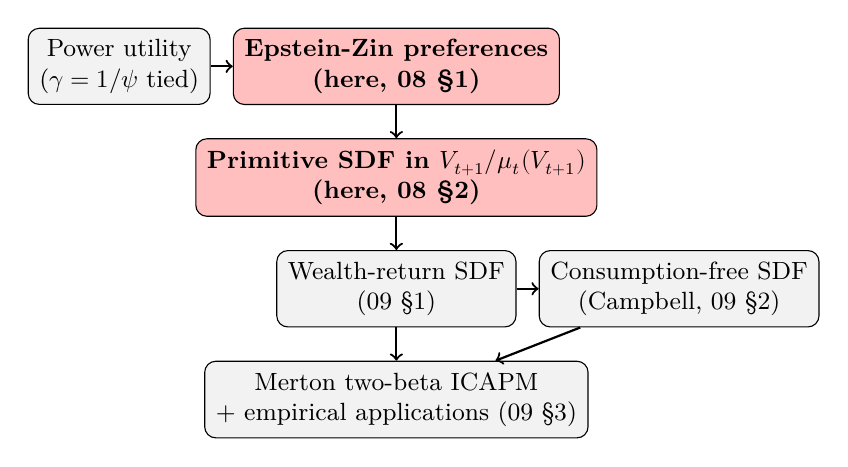
\begin{tikzpicture}[node distance=8pt,
			box/.style={draw,rounded corners,align=center,inner sep=4pt,minimum height=22pt,font=\small},
			stage/.style={box,fill=gray!10},
			here/.style={box,fill=red!25}]
			\node[stage] (a) {Power utility \\ ($\gamma=1/\psi$ tied)};
			\node[here, right=of a] (b) {\textbf{Epstein-Zin preferences} \\ \textbf{(here, 08 \S1)}};
			\node[here, below=12pt of b] (c) {\textbf{Primitive SDF in $V_{t+1}/\mu_t(V_{t+1})$} \\ \textbf{(here, 08 \S2)}};
			\node[stage, below=12pt of c] (d) {Wealth-return SDF \\ (09 \S1)};
			\node[stage, right=of d] (e) {Consumption-free SDF \\ (Campbell, 09 \S2)};
			\node[stage, below=12pt of d] (f) {Merton two-beta ICAPM \\ + empirical applications (09 \S3)};
			\draw[->,thick] (a) -- (b);
			\draw[->,thick] (b) -- (c);
			\draw[->,thick] (c) -- (d);
			\draw[->,thick] (d) -- (e);
			\draw[->,thick] (d) -- (f);
			\draw[->,thick] (e) -- (f);
		\end{tikzpicture}
	\end{center}
	\vspace{4pt}
	\begin{block}{What 08 delivers, what 09 needs}
		\begin{itemize}
			\item This lecture (08) gives you the SDF in its \textbf{primitive form}: \\
			$M_{t+1} = \delta\bigl(\tfrac{C_{t+1}}{C_t}\bigr)^{-1/\psi}\bigl(\tfrac{V_{t+1}}{\mu_t(V_{t+1})}\bigr)^{-(\gamma-1/\psi)}$ \quad --- but $V_{t+1}$ is \textbf{not observable}.
			\item Lecture 09 makes the SDF operational by replacing $V_{t+1}$ first with the wealth return, then with Campbell's consumption-free expansion.
		\end{itemize}
	\end{block}
\end{frame}

\begin{frame}{Lecture 08 Outline}
	\begin{enumerate}
		\item \textbf{Section 1.} Why the standard CRRA utility cannot solve the equity premium and risk-free rate puzzles simultaneously $\rightarrow$ recursive preferences (Kreps-Porteus, Epstein-Zin) decouple risk aversion $\gamma$ from intertemporal substitution $\psi$.
		\item \textbf{Section 2.} The chain-rule derivation of the Epstein-Zin SDF.
		\begin{itemize}
			\item Three partial derivatives: $\partial f/\partial\mu$ (driven by $\psi$), $\partial\mu/\partial V$ (driven by $\gamma$), $\partial V/\partial C$ (driven by $\psi$).
			\item Combining them yields the primitive SDF and the two-shock decomposition $\widetilde{m}_{t+1} = -\gamma\,\widetilde{c}_{t+1} - (\gamma-1/\psi)(\widetilde{v}_{t+1}-\widetilde{c}_{t+1})$.
		\end{itemize}
	\end{enumerate}
	\vspace{4pt}
	\begin{center}
		\footnotesize \textit{Goal: by the end of 08 you can write down the SDF; by the end of 09 you can take it to data.}
	\end{center}
\end{frame}

% ============================================================================
% Section: Epstein-Zin Preferences (renamed from "From Power Utility...")
% ============================================================================

\section{Epstein-Zin Preferences}

\begin{frame}
    \frametitle{The Problems with Standard Power Utility}
    
    \textbf{Standard Time-Separable CRRA Utility:}
    \begin{equation*}
        U = E_0 \sum_{t=0}^{\infty} \beta^t \frac{C_t^{1-\gamma}}{1-\gamma}
    \end{equation*}
    
    
    \textbf{Key Feature:} Single parameter $\gamma$ controls BOTH:
    \begin{itemize}
        \item Risk aversion: How much you dislike consumption volatility
        \item Intertemporal substitution: Willingness to shift consumption across time
    \end{itemize}
    
    
    \textbf{The Problem: These Are Different Concepts!}
    \begin{itemize}
        \item \textbf{Risk aversion:} Static concept about gambles at a point in time
        \begin{itemize}
            \item Example: Would you accept a 50-50 bet of \$100 vs. \$0?
        \end{itemize}
        \item \textbf{IES:} Dynamic concept about timing of consumption
        \begin{itemize}
            \item Example: Would you save more if interest rates rise?
        \end{itemize}
    \end{itemize}
    
    
    \textit{No reason these should be tied together, but CRRA forces $\gamma = 1/\psi$}  
\end{frame}

\begin{frame}
    \frametitle{Why the Constraint $\gamma = 1/\psi$ Matters}
    
    \textbf{Recall the Risk-Free Rate:}
    \begin{align*}
    &\mathrm{E}_t\left[r_{i, t+1}-r_{f, t+1}\right]+\frac{\sigma_i^2}{2}=\gamma \sigma_{i c}\\
    &r_{f,t+1} = \underbrace{-\log \beta}_{\substack{\text{Time} \\ \text{preference}}} + \underbrace{\gamma E_t[\Delta c_{t+1}]}_{\substack{\text{Intertemporal} \\ \text{substitution} \\ \text{Also } 1/\psi}} - \underbrace{\frac{\gamma^2 \sigma_{\Delta c}^2}{2}}_{\substack{\text{Precautionary} \\ \text{savings}}}
    \end{align*}

    
    \textbf{The Problem:}
    \begin{itemize}
        \item To get low $r_f$: Need small coefficient on $E[\Delta c]$ (high IES, i.e., low $\gamma$)
        \item To get high equity premium: Need high $\gamma$ (high risk aversion)
        \item But power utility forces $\gamma = 1/\psi$ $\rightarrow$ \textcolor{red}{Contradiction!}
    \end{itemize}
    
    
    \textbf{What We Want:}
    \begin{itemize}
        \item \textbf{High $\gamma$} (say, 7-10): To generate large equity premium
        \begin{itemize}
            \item Agents very averse to consumption volatility
        \end{itemize}
        \item \textbf{High $\psi$} (say, 1.5-2): To keep $r_f$ low
        \begin{itemize}
            \item Agents willing to substitute consumption intertemporally
        \end{itemize}
    \end{itemize}
    
    
    \textit{Need a preference structure that separates $\gamma$ from $\psi$!}
    
\end{frame}

\begin{frame}
    \frametitle{The Solution: Recursive Preferences}
    
    \textbf{Key Insight (\href{https://doi.org/10.2307/1913656}{\textcolor{blue}{Kreps-Porteus (1978)}}; \href{https://doi.org/10.2307/1913778}{\textcolor{blue}{Epstein and Zin (1989)}} ;\href{https://www.journals.uchicago.edu/doi/10.1086/261750} {\textcolor{blue}{Epstein and Zin (1991)}})}:
    
    Break the lifetime utility problem into two stages:
    
    
    \textbf{Stage 1: Deal with Risk} (Certainty Equivalent)
    \begin{itemize}
        \item Given stochastic future utility $U_{t+1}$, what is the certain equivalent?
        \item Use a function $\mu(U_{t+1})$ to convert random $U_{t+1}$ to certain $\bar{U}_{t+1}$
        \item This function encodes \textbf{risk aversion} (parameter $\gamma$)
    \end{itemize}
    
    
    \textbf{Stage 2: Aggregate Over Time} (Time Aggregator)
    \begin{itemize}
        \item Given current consumption $C_t$ and certain future utility $\bar{U}_{t+1}$
        \item Use a function $f(C_t, \bar{U}_{t+1})$ to aggregate
        \item This function encodes \textbf{intertemporal substitution} (parameter $\psi$)
    \end{itemize}
    
    
    \textbf{Combined:}
    \begin{equation*}
        \boxed{
        U_t = f(C_t, \mu(U_{t+1}))
        }
    \end{equation*}
    
    
    \textit{$\gamma$ and $\psi$ now appear in different functions $\rightarrow$ Can be set independently!}
    
\end{frame}

\begin{frame}
    \frametitle{Simple Two-Period Example}
    
    \textbf{Setup:}
    \begin{itemize}
        \item Consume $C_0$ at time 0 (certain)
        \item Consume stochastic $C_1$ at time 1
    \end{itemize}
    
    
    \textbf{Step 1: Certainty Equivalent of $C_1$}
    
    Question: What certain consumption $\bar{C}_1$ makes you indifferent to the lottery $C_1$?
    
    Define: $\bar{C}_1 = m(C_1)$ where $m(\cdot)$ is certainty equivalent function
    
    
    \textbf{Risk Aversion:}
    \begin{itemize}
        \item If $m(C_1) < E[C_1]$: Risk averse (prefer certain to gamble)
        \item If $m(C_1) = E[C_1]$: Risk neutral
        \item Degree of gap determined by parameter $\gamma$
    \end{itemize}
    
    
    \textbf{Step 2: Aggregate $(C_0, \bar{C}_1)$ Over Time}
    
    Define: $V = W(C_0, \bar{C}_1)$ where $W(\cdot, \cdot)$ is time aggregator
    
    
    \textbf{Intertemporal Substitution:}
    \begin{itemize}
        \item How willing to trade $C_0$ for $\bar{C}_1$?
        \item Elasticity determined by parameter $\psi$
    \end{itemize}
    
\end{frame}

\begin{frame}
    \frametitle{Two-Period Example: Mathematical Form}
    
    \textbf{Complete Preference Specification:}
    \begin{equation*}
        U = W(C_0, m(C_1))
    \end{equation*}
    
    
    \textbf{Specific Functional Forms (Epstein-Zin):}
    
    
    \textbf{1. Certainty Equivalent (CRRA):}
    \begin{equation*}
        m(C_1) = \left( E[C_1^{1-\gamma}] \right)^{\frac{1}{1-\gamma}}
    \end{equation*}
    Parameter $\gamma$: Risk aversion
    
    
    \textbf{2. Time Aggregator (CES):}
    \begin{equation*}
        W(C_0, \bar{C}_1) = \left[ (1-\delta)C_0^{1-1/\psi} + \delta \bar{C}_1^{1-1/\psi} \right]^{\frac{1}{1-1/\psi}}
    \end{equation*}
    Parameter $\psi$: Elasticity of intertemporal substitution
    
    
    \textbf{Key Feature:}
    \begin{itemize}
        \item $\gamma$ and $\psi$ are \textit{independent} parameters
        \item Can set $\gamma = 10$ (high risk aversion) and $\psi = 2$ (high IES)
        \item Not possible with standard power utility!
    \end{itemize}
    
\end{frame}

\begin{frame}
    \frametitle{Generalization to Infinite Horizon}
    
    \textbf{Recursive Formulation (\href{https://doi.org/10.2307/1913778}{\textcolor{blue}{Epstein and Zin, 1989}} ):}
    
    \begin{tcolorbox}[colback=blue!5!white, colframe=blue!75!black, title=Recursive Utility]
    \begin{equation*}
        U_t = f(C_t, \mu(U_{t+1}))
    \end{equation*}
    \end{tcolorbox}
    
    
    where:
    \begin{itemize}
        \item $U_t$: Lifetime utility from time $t$ onward
        \item $C_t$: Current consumption
        \item $U_{t+1}$: Random continuation utility (depends on future states)
        \item $\mu(\cdot)$: Certainty equivalent function (deals with risk)
        \item $f(\cdot, \cdot)$: Time aggregator (deals with intertemporal tradeoff)
    \end{itemize}
    
    
    \textbf{Why ``Recursive"?}
    \begin{itemize}
        \item Utility $U_t$ defined in terms of itself (via $U_{t+1}$)
        \item Solves forward from any point in time
        \item Alternative to time-separable expected utility
    \end{itemize}
    
\end{frame}

\begin{frame}
    \frametitle{Specific Functional Forms}
    
    \textbf{1. Certainty Equivalent Function:}
    \begin{equation*}
        \mu(U_{t+1}) = \left( E_t[U_{t+1}^{1-\gamma}] \right)^{\frac{1}{1-\gamma}}
    \end{equation*}
    
    \begin{itemize}
        \item CRRA form: If $U_{t+1}$ is lognormal, this is $\exp(E[\log U_{t+1}] - \frac{\gamma}{2}\text{Var}[\log U_{t+1}])$
        \item Parameter $\gamma > 0$: Coefficient of relative risk aversion
        \item Higher $\gamma$ $\rightarrow$ Lower certainty equivalent (more risk averse)
        \item Special case: $\gamma = 0$ gives $\mu = E[U_{t+1}]$ (risk neutral)
    \end{itemize}
    
    
    \textbf{2. Time Aggregator Function (CES):}
    \begin{equation*}
        f(C_t, \mu_t) = \left[ (1-\delta)C_t^{1-1/\psi} + \delta \mu_t^{1-1/\psi} \right]^{\frac{1}{1-1/\psi}}
    \end{equation*}
    
    \begin{itemize}
        \item CES (constant elasticity of substitution) form
        \item Parameter $\psi > 0$: Elasticity of intertemporal substitution
        \item Higher $\psi$ $\rightarrow$ More willing to substitute across time
        \item Special case: $\psi = 1$ gives Cobb-Douglas $C_t^{1-\delta} \mu_t^{\delta}$
    \end{itemize}
    
\end{frame}

\begin{frame}[shrink=18]
    \frametitle{The Complete Epstein-Zin Utility}
    
    \textbf{Putting It Together:}
    
    \begin{equation*}
        U_t = f(C_t, \mu(U_{t+1}))
    \end{equation*}
    
    Substitute the specific forms:
    
    \begin{tcolorbox}[colback=green!5!white, colframe=green!75!black, title=Epstein-Zin Utility Function]
    \begin{equation*}
        U_t = \left\{ (1-\delta)C_t^{1-1/\psi} + \delta \left[ E_t(U_{t+1}^{1-\gamma}) \right]^{\frac{1-1/\psi}{1-\gamma}} \right\}^{\frac{1}{1-1/\psi}}
    \end{equation*}
    \end{tcolorbox}
    
    
    \textbf{Parameters:}
    \begin{itemize}
        \item $\delta \in (0,1)$: Time discount factor
        \item $\gamma > 0$: Coefficient of relative risk aversion (RRA)
        \item $\psi > 0$: Elasticity of intertemporal substitution (EIS)
    \end{itemize}
    
    
    \textbf{Key Feature:}
    \begin{equation*}
        \text{In power utility: } \gamma = \frac{1}{\psi} \quad \text{(forced)}
    \end{equation*}
    \begin{equation*}
        \text{In Epstein-Zin: } \gamma \neq \frac{1}{\psi} \quad \text{(flexible)}
    \end{equation*}
    
\end{frame}

\begin{frame}[allowframebreaks]
    \frametitle{Alternative Parameterization}
    
    \textbf{First define two shorthand parameters:}
    \begin{equation*}
        \rho \equiv 1-\frac{1}{\psi}, \qquad \alpha \equiv 1-\gamma
    \end{equation*}
    
    Then the Epstein-Zin utility can be written as
    \begin{equation*}
        U_t=\left[(1-\delta)C_t^\rho+\delta\left(E_tU_{t+1}^{\alpha}\right)^{\rho/\alpha}\right]^{1/\rho}.
    \end{equation*}
    
    \textbf{The composite parameter used in Lecture 09 is:}
    \begin{equation*}
        \boxed{\theta \equiv \frac{1-\gamma}{1-1/\psi}=\frac{\alpha}{\rho}}
    \end{equation*}
    
    \begin{block}{Why introduce $\theta$?}
        $\theta$ is not a new preference primitive. It is a bookkeeping device that makes the SDF algebra compact. In Lecture 09 it lets us write the wealth-return SDF as
        \[
        M_{t+1}=\delta^\theta\left(\frac{C_{t+1}}{C_t}\right)^{-\theta/\psi}(1+R_{W,t+1})^{-(1-\theta)}.
        \]
    \end{block}

    \framebreak

    \textbf{Equivalent utility representation.}
    Since
    \begin{equation*}
        \rho=\frac{1-\gamma}{\theta}, \qquad \frac{\rho}{1-\gamma}=\frac{1}{\theta}, \qquad \frac{1}{\rho}=\frac{\theta}{1-\gamma},
    \end{equation*}
    we can rewrite utility as
    \begin{tcolorbox}[colback=green!5!white, colframe=green!75!black, title=Equivalent Epstein-Zin Form]
    \begin{equation*}
        U_t=
        \left[
        (1-\delta)C_t^{(1-\gamma)/\theta}
        +\delta\left(E_tU_{t+1}^{1-\gamma}\right)^{1/\theta}
        \right]^{\theta/(1-\gamma)}.
    \end{equation*}
    \end{tcolorbox}

    \textbf{The identity we will use repeatedly:}
    \begin{equation*}
        \boxed{\gamma-\frac{1}{\psi}=(1-\theta)\left(1-\frac{1}{\psi}\right)=(1-\theta)\rho}
    \end{equation*}

    \framebreak
    
    \textbf{Interpretation of $\theta$:}
    \begin{itemize}
        \item $\theta$ summarizes the relative strength of risk aversion and intertemporal substitution.
        \item If $\gamma = 1/\psi$, then $\theta=1$ and Epstein-Zin collapses to standard CRRA.
        \item If $\gamma \neq 1/\psi$, the SDF contains an additional continuation-value or wealth-return component.
        \item Do \textbf{not} read the sign of $\theta$ mechanically as a timing preference. For example, when $\gamma>1$ and $\psi>1$, $\theta<0$ under this convention, but $\gamma>1/\psi$ still means risk aversion is strong relative to IES.
    \end{itemize}
    
    
    \textbf{Economic Intuition:}
    \begin{itemize}
        \item The economically meaningful comparison is $\gamma$ versus $1/\psi$.
        \item If $\gamma > 1/\psi$: risk aversion is high relative to IES, so continuation-value risk matters for asset prices.
        \item This is exactly why the primitive SDF will contain the extra term
        \[
            \left(\frac{V_{t+1}}{\mu_t(V_{t+1})}\right)^{-(\gamma-1/\psi)}.
        \]
    \end{itemize}
    
\end{frame}

\begin{frame}
    \frametitle{Special Cases: Nesting Standard Preferences}
    
    \textbf{1. Expected Utility ($\gamma = 1/\psi$):}
    
    When $\theta = 1$:
    \begin{equation*}
        U_t = E_t \sum_{s=0}^{\infty} \delta^s \frac{C_{t+s}^{1-\gamma}}{1-\gamma}
    \end{equation*}
    Standard time-separable CRRA utility
    
    
    \textbf{2. Risk Neutrality ($\gamma = 0$):}
    \begin{equation*}
        U_t = \left[ (1-\delta)C_t^{1-1/\psi} + \delta (E_t U_{t+1})^{1-1/\psi} \right]^{\frac{1}{1-1/\psi}}
    \end{equation*}
    Only IES matters, no risk aversion
    
    
    \textbf{3. Log Utility ($\gamma = 1$ and $\psi = 1$):}
    \begin{equation*}
        U_t = (1-\delta) \log C_t + \delta E_t[U_{t+1}]
    \end{equation*}
    Linear in expectations (tractable)
    
\end{frame}

\begin{frame}
    \frametitle{Why Epstein-Zin Helps with Asset Pricing Puzzles}
    
    \textbf{The Flexibility:}
    
    Can now choose:
    \begin{itemize}
        \item $\gamma = 7.5$: High risk aversion (generates large equity premium)
        \item $\psi = 1.5$: High IES, so $1/\psi = 0.67$ (keeps $r_f$ low)
    \end{itemize}
    
    
    \textbf{Risk-Free Rate:}
    \begin{equation*}
        r_f \approx -\log \delta + \frac{1}{\psi} E[\Delta c] - \frac{1}{2\psi^2} \sigma_{\Delta c}^2 + \text{other terms}
    \end{equation*}
    With $\psi = 1.5$, coefficient on $E[\Delta c]$ is $0.67$ instead of $7.5$ $\rightarrow$ Much lower $r_f$!
    
    
    \textbf{Equity Premium:}
    \begin{itemize}
        \item SDF includes term: $(V_{t+1}/\mu(V_{t+1}))^{-(\gamma - 1/\psi)}$
        \item With $\gamma = 7.5$, $\psi = 1.5$: Exponent is $-(7.5 - 0.67) = -6.83$
        \item Strong response to wealth shocks $\rightarrow$ Large equity premium
    \end{itemize}
    
    
    \textit{Can simultaneously match both $r_f$ and equity premium!}
    
\end{frame}

\begin{frame}
    \frametitle{Summary: From Power Utility to Epstein-Zin}
    
    \begin{table}
        \footnotesize
        \begin{tabular}{p{3cm}|p{3.5cm}|p{3.5cm}}
            \toprule
            \textbf{Feature} & \textbf{Power Utility} & \textbf{Epstein-Zin} \\
            \midrule
            Risk aversion & $\gamma$ & $\gamma$ (independent) \\[0.2cm]
            IES & $\psi = 1/\gamma$ (tied) & $\psi$ (independent) \\[0.2cm]
            Utility form & Time-separable & Recursive \\[0.2cm]
            Parameters & 1 ($\gamma$) & 2 ($\gamma, \psi$) \\[0.2cm]
            Equity premium & Need $\gamma > 30$ & Can use $\gamma \approx 7.5$ \\[0.2cm]
            Risk-free rate & Too high with high $\gamma$ & Can set via $\psi$ \\[0.2cm]
            Both puzzles & \textcolor{red}{Impossible} & \textcolor{green}{Possible!} \\
            \bottomrule
        \end{tabular}
    \end{table}
    
    
    \textbf{Bottom Line:}
    \begin{itemize}
        \item Power utility conflates two distinct economic concepts
        \item Epstein-Zin separates risk aversion from intertemporal substitution
        \item Extra flexibility resolves major asset pricing puzzles
        \item Foundation of modern macro-finance models (long-run risk, disaster risk, etc.)
    \end{itemize}
\end{frame}

% ============================================================================
% Section: The Primitive Epstein-Zin SDF
% ============================================================================
\section{The Primitive Epstein-Zin SDF}

% ============================================================================
% Section-level navigation: where each partial derivative fits
% ============================================================================
\begin{frame}[shrink=20]{Roadmap of the SDF Derivation}
	The pricing kernel is a marginal rate of substitution:
	\begin{equation*}
		q(s_t \to s_{t+1}) = \frac{\partial V_t/\partial C_{t+1}(s_t,s_{t+1})}{\partial V_t/\partial C_t(s_t)}.
	\end{equation*}
	Because $V_t = f(C_t,\mu_t(V_{t+1}))$ is recursive, we apply the chain rule:
	\vspace{4pt}
	\begin{center}
		\small
		\begin{tikzpicture}[node distance=4pt,
			box/.style={draw,rounded corners,align=center,inner sep=4pt,font=\small,minimum height=20pt}]
			\node[box,fill=blue!10] (a) {$\dfrac{\partial f}{\partial \mu(V_{t+1})}$};
			\node[box,fill=blue!10,right=of a] (b) {$\dfrac{\partial \mu(V_{t+1})}{\partial V_{t+1}(s_{t+1})}$};
			\node[box,fill=blue!10,right=of b] (c) {$\dfrac{\partial V_{t+1}}{\partial C_{t+1}(s_{t+1})}$};
			\draw[->,thick] (a) -- (b);
			\draw[->,thick] (b) -- (c);
		\end{tikzpicture}
	\end{center}
	\vspace{2pt}
	\begin{center}
		\small
		\begin{tabular}{@{}llc@{}}
			\toprule
			\textbf{Partial} & \textbf{Driving parameter} & \textbf{Frame in this section} \\
			\midrule
			$\partial f/\partial\mu(V_{t+1})$ & EIS $\psi$ (time aggregator) & PD~1 \\
			$\partial\mu/\partial V_{t+1}$ & risk aversion $\gamma$ (CE function) & PD~2 \\
			$\partial V_{t+1}/\partial C_{t+1}$ & EIS $\psi$ (time aggregator at $t{+}1$) & PD~3 \\
			$\partial V_t/\partial C_t$ & EIS $\psi$ (denominator) & Den. \\
			\bottomrule
		\end{tabular}
	\end{center}
	\vspace{2pt}
	\begin{block}{Output of this section}
		Combining the four partials gives the primitive Epstein-Zin SDF
		$M_{t+1} = \delta\bigl(\tfrac{C_{t+1}}{C_t}\bigr)^{-1/\psi}\bigl(\tfrac{V_{t+1}}{\mu_t(V_{t+1})}\bigr)^{-(\gamma-1/\psi)}$.
		The unobservability of $V_{t+1}$ motivates the operationalization in Lecture~09.
	\end{block}
\end{frame}

% ============================================================================
% Detailed Derivation: Epstein-Zin SDF
% ============================================================================

\begin{frame}[allowframebreaks]
    \frametitle{Deriving the SDF: Setup and Intuition}
    
    \textbf{Our goal:} Derive the stochastic discount factor (SDF) for an agent with Epstein-Zin preferences.
    
    \textbf{Key idea:} The SDF equals the marginal rate of substitution between consumption today and consumption tomorrow.
    
    \textbf{Recall the recursive utility specification:}
    \begin{equation*}
        V_t = f(C_t, \mu_t(V_{t+1}))
    \end{equation*}
    
    This says: lifetime utility today depends on current consumption $C_t$ and expected future utility $\mu_t(V_{t+1})$.
    
    \framebreak
    
    \textbf{The two building blocks:}
    
    \textbf{1. Time aggregator:} Combines current consumption with continuation utility
    \begin{equation*}
        f(C, v) = \left[ (1-\delta)C^{1-1/\psi} + \delta v^{1-1/\psi} \right]^{\frac{1}{1-1/\psi}}
    \end{equation*}
    \begin{itemize}
        \item Parameter $\psi$: elasticity of intertemporal substitution (EIS)
        \item Controls willingness to substitute consumption across time
        \item Homogeneous of degree 1 (scales with wealth)
    \end{itemize}
    
    \framebreak
    
    \textbf{2. Certainty equivalent:} Aggregates uncertain future utilities
    \begin{equation*}
        \mu_t(V_{t+1}) = \left[ \sum_{s_{t+1}|s_t} \pi(s_t \to s_{t+1})V_{t+1}(s_t, s_{t+1})^{1-\gamma} \right]^{\frac{1}{1-\gamma}}
    \end{equation*}
    \begin{itemize}
        \item Parameter $\gamma$: coefficient of relative risk aversion
        \item Controls attitude toward risk in continuation utility
        \item When $\gamma > 0$: risk averse in continuation utility
        \item When $\gamma = 0$: risk neutral in continuation utility
        \item When $\gamma = 1$: log-utility limit of the certainty equivalent
    \end{itemize}
    
    \textbf{Key insight:} By separating $\psi$ and $\gamma$, we decouple intertemporal substitution from risk aversion.
    
    \framebreak
    
    \textbf{The marginal rate of substitution approach:}
    
    The pricing kernel (state price) measures the rate at which the agent is willing to trade consumption today for consumption tomorrow in a specific state:
    \begin{equation*}
        q(s_t \to s_{t+1}) = \frac{\partial V_t/\partial C_{t+1}(s_t, s_{t+1})}{\partial V_t/\partial C_t(s_t)}
    \end{equation*}
    
    \textbf{Economic interpretation:}
    \begin{itemize}
        \item \textbf{Numerator:} Marginal value of receiving an extra unit of consumption tomorrow in state $s_{t+1}$, measured in units of lifetime utility today
        \item \textbf{Denominator:} Marginal value of consuming an extra unit today, measured in units of lifetime utility today
        \item \textbf{Ratio:} How many units of consumption today the agent would give up for one unit tomorrow in state $s_{t+1}$
    \end{itemize}
    
    \framebreak
    
    \textbf{Why is the numerator complicated?}
    
    To compute $\frac{\partial V_t}{\partial C_{t+1}(s_t, s_{t+1})}$, we need to trace how consumption at $t+1$ affects utility at time $t$ through the recursive structure:
    
    \begin{equation*}
        C_{t+1} \to V_{t+1} \to \mu_t(V_{t+1}) \to V_t
    \end{equation*}
    
    \textbf{Chain rule decomposition:}
    \begin{equation*}
        \frac{\partial V_t}{\partial C_{t+1}(s_t, s_{t+1})} = \underbrace{\frac{\partial f}{\partial \mu(V_{t+1})}}_{\text{Step 1}} \cdot \underbrace{\frac{\partial \mu(V_{t+1})}{\partial V_{t+1}(s_t, s_{t+1})}}_{\text{Step 2}} \cdot \underbrace{\frac{\partial V_{t+1}(s_t, s_{t+1})}{\partial C_{t+1}(s_t, s_{t+1})}}_{\text{Step 3}}
    \end{equation*}
    
    \framebreak
    
    \textbf{Roadmap for the derivation:}
    
    We will compute each partial derivative separately:
    
    \textbf{Step 1:} $\frac{\partial f}{\partial \mu(V_{t+1})}$
    \begin{itemize}
        \item How does current lifetime utility respond to changes in expected continuation utility?
        \item Involves the time aggregator function
        \item Key parameter: $\psi$ (EIS)
    \end{itemize}
    
    \textbf{Step 2:} $\frac{\partial \mu(V_{t+1})}{\partial V_{t+1}(s_t, s_{t+1})}$
    \begin{itemize}
        \item How does expected continuation utility respond to realized utility in a specific state?
        \item Involves the certainty equivalent function
        \item Key parameter: $\gamma$ (risk aversion)
    \end{itemize}
    
    \textbf{Step 3:} $\frac{\partial V_{t+1}(s_t, s_{t+1})}{\partial C_{t+1}(s_t, s_{t+1})}$
    \begin{itemize}
        \item How does tomorrow's lifetime utility respond to tomorrow's consumption?
        \item Similar to Step 1, but evaluated at $t+1$
        \item Also involves parameter $\psi$
    \end{itemize}
    
    \framebreak
    
    \textbf{Finally:} We will also compute the denominator
    \begin{equation*}
        \frac{\partial V_t}{\partial C_t(s_t)}
    \end{equation*}
    which measures the marginal value of consumption today.
    
    \textbf{Then:} Form the ratio to get the pricing kernel, and normalize by probability to obtain the SDF.
    
    \textbf{The beauty of this approach:} Each partial derivative has clear economic interpretation, and together they reveal how both intertemporal substitution and risk aversion determine asset prices.
\end{frame}

\begin{frame}[allowframebreaks]
    \frametitle{Partial Derivative 1: $\frac{\partial f}{\partial \mu(V_{t+1})}$}
    
    \textbf{Starting from:}
    \begin{equation*}
        f(C_t, \mu(V_{t+1})) = \left[ (1-\delta)C_t^{1-1/\psi} + \delta\mu(V_{t+1})^{1-1/\psi} \right]^{\frac{1}{1-1/\psi}}
    \end{equation*}
    
    \textbf{Taking partial derivative with respect to $\mu(V_{t+1})$:}
    
    Using the chain rule with $g(x) = x^{1/(1-1/\psi)}$ and $h(\mu) = (1-\delta)C_t^{1-1/\psi} + \delta\mu^{1-1/\psi}$:
    \begin{equation*}
        \frac{\partial f}{\partial \mu} = g'(h(\mu)) \cdot h'(\mu)
    \end{equation*}
    
    \framebreak
    
    \textbf{Step 1: Compute $g'(h)$}
    \begin{equation*}
        g'(h) = \frac{1}{1-1/\psi} h^{\frac{1}{1-1/\psi}-1}
    \end{equation*}
    
    \textbf{Step 2: Compute $h'(\mu)$}
    \begin{equation*}
        h'(\mu) = \delta \left(1 - \frac{1}{\psi}\right) \mu(V_{t+1})^{1-1/\psi-1} = \delta \left(1 - \frac{1}{\psi}\right) \mu(V_{t+1})^{-1/\psi}
    \end{equation*}
    
    \framebreak
    
    \textbf{Step 3: Multiply the terms}
    \begin{equation*}
        \begin{aligned}
            \frac{\partial f}{\partial \mu(V_{t+1})} &= \frac{1}{1-1/\psi} \left[ (1-\delta)C_t^{1-1/\psi} + \delta\mu(V_{t+1})^{1-1/\psi} \right]^{\frac{1}{1-1/\psi}-1} \\
            &\quad \times \delta \left(1 - \frac{1}{\psi}\right) \mu(V_{t+1})^{-1/\psi}
        \end{aligned}
    \end{equation*}
    
    \framebreak
    
    \textbf{Step 4: Simplify the exponent}
    
    Note that:
    \begin{equation*}
        \frac{1}{1-1/\psi} - 1 = \frac{1 - (1-1/\psi)}{1-1/\psi} = \frac{1/\psi}{1-1/\psi}
    \end{equation*}
    
    Also note that:
    \begin{equation*}
        \left(1 - \frac{1}{\psi}\right) \cdot \frac{1}{1-1/\psi} = 1
    \end{equation*}
    
    \framebreak
    
    \textbf{Step 5: Apply simplifications}
    \begin{equation*}
        \begin{aligned}
            \frac{\partial f}{\partial \mu(V_{t+1})} &= \left[ (1-\delta)C_t^{1-1/\psi} + \delta\mu(V_{t+1})^{1-1/\psi} \right]^{\frac{1/\psi}{1-1/\psi}} \\
            &\quad \times \delta \mu(V_{t+1})^{-1/\psi}
        \end{aligned}
    \end{equation*}
    
    \textbf{Step 6: Recognize $f(C_t, \mu(V_{t+1})) = V_t$}
    \begin{equation*}
        \left[ (1-\delta)C_t^{1-1/\psi} + \delta\mu(V_{t+1})^{1-1/\psi} \right]^{\frac{1}{1-1/\psi}} = V_t
    \end{equation*}
    
    Therefore:
    \begin{equation*}
        \left[ (1-\delta)C_t^{1-1/\psi} + \delta\mu(V_{t+1})^{1-1/\psi} \right]^{\frac{1/\psi}{1-1/\psi}} = V_t^{1/\psi}
    \end{equation*}
    
    \framebreak
    
    \textbf{Final result:}
    \begin{tcolorbox}[colback=blue!5!white, colframe=blue!75!black, title=Partial Derivative 1]
    \begin{equation*}
        \frac{\partial f(C_t, \mu(V_{t+1}))}{\partial \mu(V_{t+1})} = \delta V_t^{1/\psi} \mu(V_{t+1})^{-1/\psi}
    \end{equation*}
    \end{tcolorbox}
    
    \textbf{Economic interpretation:}
    \begin{itemize}
        \item Measures how current lifetime utility $V_t$ responds to changes in expected future utility
        \item Higher $\psi$ (EIS) reduces sensitivity to future utility changes
        \item The factor $\delta$ reflects time discounting
    \end{itemize}
\end{frame}

\begin{frame}[allowframebreaks]
    \frametitle{Partial Derivative 2: $\frac{\partial \mu(V_{t+1})}{\partial V_{t+1}(s_t, s_{t+1})}$}
    
    \textbf{Starting from:}
    \begin{equation*}
        \mu(V_{t+1}) = \left[ \sum_{s_{t+1}|s_t} \pi(s_t \to s_{t+1})V_{t+1}(s_t, s_{t+1})^{1-\gamma} \right]^{\frac{1}{1-\gamma}}
    \end{equation*}
    
    \textbf{Taking partial derivative with respect to $V_{t+1}(s_t, s_{t+1})$ for a specific state:}
    
    Using the chain rule with $g(x) = x^{1/(1-\gamma)}$ and $h(V_{t+1}) = \sum_{s_{t+1}} \pi V_{t+1}^{1-\gamma}$:
    \begin{equation*}
        \frac{\partial \mu}{\partial V_{t+1}} = g'(h) \cdot \frac{\partial h}{\partial V_{t+1}}
    \end{equation*}
    
    \framebreak
    
    \textbf{Step 1: Compute $g'(h)$}
    \begin{equation*}
        g'(h) = \frac{1}{1-\gamma} h^{\frac{1}{1-\gamma}-1}
    \end{equation*}
    
    \textbf{Step 2: Compute $\frac{\partial h}{\partial V_{t+1}(s_t, s_{t+1})}$}
    
    When taking the derivative of the sum with respect to $V_{t+1}$ in a specific state, only that term survives:
    \begin{equation*}
    \begin{aligned}
       & \frac{\partial}{\partial V_{t+1}(s_t, s_{t+1})} \left[ \sum_{s_{t+1}|s_t} \pi(s_t \to s_{t+1})V_{t+1}(s_t, s_{t+1})^{1-\gamma} \right] \\
   = & \pi(s_t \to s_{t+1})(1-\gamma)V_{t+1}(s_t, s_{t+1})^{-\gamma}
    \end{aligned} 
    \end{equation*}
    
    \framebreak
    
    \textbf{Step 3: Multiply the terms}
    \begin{equation*}
        \begin{aligned}
            \frac{\partial \mu(V_{t+1})}{\partial V_{t+1}(s_t, s_{t+1})} &= \frac{1}{1-\gamma} \left[ \sum_{s_{t+1}|s_t} \pi(s_t \to s_{t+1})V_{t+1}(s_t, s_{t+1})^{1-\gamma} \right]^{\frac{1}{1-\gamma}-1} \\
            &\quad \times \pi(s_t \to s_{t+1})(1-\gamma)V_{t+1}(s_t, s_{t+1})^{-\gamma}
        \end{aligned}
    \end{equation*}
    
    \framebreak
    
    \textbf{Step 4: Simplify}
    
    The $(1-\gamma)$ terms cancel:
    \begin{equation*}
        \begin{aligned}
            \frac{\partial \mu(V_{t+1})}{\partial V_{t+1}(s_t, s_{t+1})} &= \left[ \sum_{s_{t+1}|s_t} \pi(s_t \to s_{t+1})V_{t+1}(s_t, s_{t+1})^{1-\gamma} \right]^{\frac{1}{1-\gamma}-1} \\
            &\quad \times \pi(s_t \to s_{t+1})V_{t+1}(s_t, s_{t+1})^{-\gamma}
        \end{aligned}
    \end{equation*}
    
    \framebreak
    
    \textbf{Step 5: Simplify the exponent}
    
    Note that:
    \begin{equation*}
        \frac{1}{1-\gamma} - 1 = \frac{1 - (1-\gamma)}{1-\gamma} = \frac{\gamma}{1-\gamma}
    \end{equation*}
    
    Therefore:
    \begin{equation*}
        \left[ \sum_{s_{t+1}|s_t} \pi(s_t \to s_{t+1})V_{t+1}(s_t, s_{t+1})^{1-\gamma} \right]^{\frac{\gamma}{1-\gamma}} = \mu(V_{t+1})^{\gamma}
    \end{equation*}
    
    \framebreak
    
    \textbf{Final result:}
    \begin{tcolorbox}[colback=blue!5!white, colframe=blue!75!black, title=Partial Derivative 2]
    \begin{equation*}
        \frac{\partial \mu(V_{t+1})}{\partial V_{t+1}(s_t, s_{t+1})} = \mu(V_{t+1})^{\gamma} \pi(s_t \to s_{t+1}) V_{t+1}(s_t, s_{t+1})^{-\gamma}
    \end{equation*}
    \end{tcolorbox}
    
    \textbf{Economic interpretation:}
    \begin{itemize}
        \item Measures how expected continuation utility responds to realized utility in a specific state
        \item Higher $\gamma$ (risk aversion) increases the weight on deviations from expectation
        \item The probability $\pi$ weights states by their likelihood
    \end{itemize}
\end{frame}

\begin{frame}[allowframebreaks]
    \frametitle{Partial Derivative 3: $\frac{\partial V_{t+1}(s_t, s_{t+1})}{\partial C_{t+1}(s_t, s_{t+1})}$}
    
    \textbf{Starting from:}
    \begin{equation*}
        V_{t+1}(s_t, s_{t+1}) = f(C_{t+1}(s_t, s_{t+1}), \mu_{t+1}(V_{t+2}))
    \end{equation*}
    
    This has the same functional form as the time aggregator at time $t$, but evaluated at $t+1$.
    
    \textbf{Taking partial derivative with respect to $c_{t+1}$:}
    \begin{equation*}
        f(C_{t+1}, \mu_{t+1}(V_{t+2})) = \left[ (1-\delta)C_{t+1}^{1-1/\psi} + \delta\mu_{t+1}(V_{t+2})^{1-1/\psi} \right]^{\frac{1}{1-1/\psi}}
    \end{equation*}
    
    \framebreak
    
    \textbf{Step 1: Apply chain rule}
    
    Using the same approach as Partial Derivative 1, but now with respect to consumption:
    \begin{equation*}
        \begin{aligned}
            \frac{\partial f}{\partial C_{t+1}} &= \frac{1}{1-1/\psi} \left[ (1-\delta)C_{t+1}^{1-1/\psi} + \delta\mu_{t+1}(V_{t+2})^{1-1/\psi} \right]^{\frac{1}{1-1/\psi}-1} \\
            &\quad \times (1-\delta) \left(1 - \frac{1}{\psi}\right) C_{t+1}^{1-1/\psi-1}
        \end{aligned}
    \end{equation*}
    
    \framebreak
    
    \textbf{Step 2: Simplify the exponent on $C_{t+1}$}
    \begin{equation*}
        1 - \frac{1}{\psi} - 1 = -\frac{1}{\psi}
    \end{equation*}
    
    So:
    \begin{equation*}
        C_{t+1}^{1-1/\psi-1} = C_{t+1}^{-1/\psi}
    \end{equation*}
    
    \framebreak
    
    \textbf{Step 3: Cancel terms}
    
    The factor $\left(1 - \frac{1}{\psi}\right) \cdot \frac{1}{1-1/\psi} = 1$, so:
    \begin{equation*}
        \begin{aligned}
            \frac{\partial f}{\partial C_{t+1}} &= \left[ (1-\delta)C_{t+1}^{1-1/\psi} + \delta\mu_{t+1}(V_{t+2})^{1-1/\psi} \right]^{\frac{1/\psi}{1-1/\psi}} \\
            &\quad \times (1-\delta) C_{t+1}^{-1/\psi}
        \end{aligned}
    \end{equation*}
    
    \framebreak
    
    \textbf{Step 4: Recognize $f(C_{t+1}, \mu_{t+1}(V_{t+2})) = V_{t+1}$}
    \begin{equation*}
        \left[ (1-\delta)C_{t+1}^{1-1/\psi} + \delta\mu_{t+1}(V_{t+2})^{1-1/\psi} \right]^{\frac{1/\psi}{1-1/\psi}} = V_{t+1}^{1/\psi}
    \end{equation*}
    
    \framebreak
    
    \textbf{Final result:}
    \begin{tcolorbox}[colback=blue!5!white, colframe=blue!75!black, title=Partial Derivative 3]
    \begin{equation*}
        \frac{\partial V_{t+1}(s_t, s_{t+1})}{\partial C_{t+1}(s_t, s_{t+1})} = V_{t+1}^{1/\psi} (1-\delta) C_{t+1}(s_t, s_{t+1})^{-1/\psi}
    \end{equation*}
    \end{tcolorbox}
    
    \textbf{Economic interpretation:}
    \begin{itemize}
        \item Marginal value of consumption tomorrow in terms of tomorrow's lifetime utility
        \item Higher $\psi$ (EIS) reduces sensitivity to consumption changes
        \item Factor $(1-\delta)$ reflects weight on current consumption in the aggregator
    \end{itemize}
\end{frame}

\begin{frame}[allowframebreaks]
    \frametitle{Denominator: $\frac{\partial V_t}{\partial C_t(s_t)}$}
    
    \textbf{Starting from:}
    \begin{equation*}
        V_t = f(C_t, \mu_t(V_{t+1}))
    \end{equation*}
    
    \textbf{This is the same functional form as Partial Derivative 3, but evaluated at time $t$:}
    
    By the exact same derivation:
    \begin{tcolorbox}[colback=blue!5!white, colframe=blue!75!black, title=Denominator]
    \begin{equation*}
        \frac{\partial V_t}{\partial C_t(s_t)} = V_t^{1/\psi} (1-\delta) C_t^{-1/\psi}
    \end{equation*}
    \end{tcolorbox}
    
    \textbf{Economic interpretation:}
    \begin{itemize}
        \item Marginal value of consumption today in terms of current lifetime utility
        \item Appears in denominator because we compute marginal rate of substitution
        \item Higher consumption today reduces its marginal value
    \end{itemize}
\end{frame}

\begin{frame}[allowframebreaks]
    \frametitle{Combining Terms: The Pricing Kernel}
    
    \textbf{Step 1: Multiply numerator terms}
    
    \begin{equation*}
        \begin{aligned}
            \frac{\partial V_t}{\partial C_{t+1}(s_t, s_{t+1})} &= \frac{\partial f}{\partial \mu(V_{t+1})} \times \frac{\partial \mu(V_{t+1})}{\partial V_{t+1}} \times \frac{\partial V_{t+1}}{\partial C_{t+1}} \\[0.3cm]
            &= \left[ \delta V_t^{1/\psi} \mu(V_{t+1})^{-1/\psi} \right] \\
            &\quad \times \left[ \mu(V_{t+1})^{\gamma} \pi(s_t \to s_{t+1}) V_{t+1}^{-\gamma} \right] \\
            &\quad \times \left[ V_{t+1}^{1/\psi} (1-\delta) C_{t+1}^{-1/\psi} \right]
        \end{aligned}
    \end{equation*}
    
    \framebreak
    
    \textbf{Step 2: Collect terms by variable}
    
    \begin{equation*}
        \begin{aligned}
            \frac{\partial V_t}{\partial C_{t+1}} &= \delta (1-\delta) \pi(s_t \to s_{t+1}) \\
            &\quad \times V_t^{1/\psi} \times \mu(V_{t+1})^{-1/\psi + \gamma} \times V_{t+1}^{-\gamma + 1/\psi} \times C_{t+1}^{-1/\psi}
        \end{aligned}
    \end{equation*}
    
    \framebreak
    
    \textbf{Step 3: Form the pricing kernel}
    
    The pricing kernel is:
    \begin{equation*}
        q(s_t \to s_{t+1}) = \frac{\partial V_t/\partial c_{t+1}}{\partial V_t/\partial C_t}
    \end{equation*}
    
    Substitute numerator and denominator:
    \begin{equation*}
        \begin{aligned}
            q(s_t \to s_{t+1}) &= \frac{\delta (1-\delta) \pi V_t^{1/\psi} \mu(V_{t+1})^{-1/\psi + \gamma} V_{t+1}^{-\gamma + 1/\psi} C_{t+1}^{-1/\psi}}{V_t^{1/\psi} (1-\delta) C_t^{-1/\psi}}
        \end{aligned}
    \end{equation*}
    
    \framebreak
    
    \textbf{Step 4: Cancel common terms}
    
    Cancel $V_t^{1/\psi}$ and $(1-\delta)$:
    \begin{equation*}
        q(s_t \to s_{t+1}) = \delta \pi(s_t \to s_{t+1}) \frac{C_{t+1}^{-1/\psi}}{C_t^{-1/\psi}} \mu(V_{t+1})^{-1/\psi + \gamma} V_{t+1}^{-\gamma + 1/\psi}
    \end{equation*}
    
    Simplify the consumption ratio:
    \begin{equation*}
        \frac{C_{t+1}^{-1/\psi}}{C_t^{-1/\psi}} = \left( \frac{C_{t+1}}{C_t} \right)^{-1/\psi}
    \end{equation*}
    
    \framebreak
    
    \textbf{Step 5: Combine powers of $\mu(V_{t+1})$ and $V_{t+1}$}
    
    \begin{equation*}
        \mu(V_{t+1})^{-1/\psi + \gamma} V_{t+1}^{-\gamma + 1/\psi} = \mu(V_{t+1})^{\gamma - 1/\psi} V_{t+1}^{1/\psi - \gamma}
    \end{equation*}
    
    Note that:
    \begin{equation*}
        V_{t+1}^{1/\psi - \gamma} = V_{t+1}^{-(\gamma - 1/\psi)}
    \end{equation*}
    
    Therefore:
    \begin{equation*}
        \mu(V_{t+1})^{\gamma - 1/\psi} V_{t+1}^{-(\gamma - 1/\psi)} = \left( \frac{\mu(V_{t+1})}{V_{t+1}} \right)^{\gamma - 1/\psi}
    \end{equation*}
    
    \framebreak
    
    \textbf{Step 6: Express as ratio}
    
    We can rewrite:
    \begin{equation*}
        \left( \frac{\mu(V_{t+1})}{V_{t+1}} \right)^{\gamma - 1/\psi} = \left( \frac{V_{t+1}}{\mu(V_{t+1})} \right)^{-(\gamma - 1/\psi)}
    \end{equation*}
    
    \framebreak
    
    \textbf{Final pricing kernel:}
    \begin{tcolorbox}[colback=green!5!white, colframe=green!75!black, title=Pricing Kernel]
    \begin{equation*}
        q(s_t \to s_{t+1}) = \delta \pi(s_t \to s_{t+1}) \left( \frac{C_{t+1}}{C_t} \right)^{-1/\psi} \left( \frac{V_{t+1}}{\mu_t(V_{t+1})} \right)^{-(\gamma - 1/\psi)}
    \end{equation*}
    \end{tcolorbox}
\end{frame}

\begin{frame}[allowframebreaks]
    \frametitle{From Pricing Kernel to SDF}
    
    \textbf{Definition of the SDF:}
    
    The stochastic discount factor is the pricing kernel normalized by the probability:
    \begin{equation*}
        M(s_t, s_{t+1}) \equiv \frac{q(s_t \to s_{t+1})}{\pi(s_t \to s_{t+1})}
    \end{equation*}
    
    \textbf{Substituting our pricing kernel:}
    \begin{equation*}
        M_{t+1} = \frac{\delta \pi(s_t \to s_{t+1}) \left( \frac{C_{t+1}}{C_t} \right)^{-1/\psi} \left( \frac{V_{t+1}}{\mu_t(V_{t+1})} \right)^{-(\gamma - 1/\psi)}}{\pi(s_t \to s_{t+1})}
    \end{equation*}
    
    \framebreak
    
    \textbf{Cancel $\pi(s_t \to s_{t+1})$:}
    
    \begin{tcolorbox}[colback=blue!5!white, colframe=blue!75!black, title=Epstein-Zin SDF (Final Form)]
    \begin{equation*}
        M_{t+1} = \delta \left( \frac{C_{t+1}}{C_t} \right)^{-1/\psi} \left( \frac{V_{t+1}}{\mu_t(V_{t+1})} \right)^{-(\gamma - 1/\psi)}
    \end{equation*}
    \end{tcolorbox}
    
    where:
    \begin{itemize}
        \item $\delta$: Time discount factor
        \item $1/\psi$: Inverse of elasticity of intertemporal substitution
        \item $\gamma$: Relative risk aversion
        \item $V_{t+1}/\mu_t(V_{t+1})$: Ratio of realized to expected continuation value
    \end{itemize}
    
    \framebreak
    
    \textbf{Verification: Special case}
    
    When $\gamma = 1/\psi$:
    \begin{equation*}
        \left( \frac{V_{t+1}}{\mu_t(V_{t+1})} \right)^{-(\gamma - 1/\psi)} = \left( \frac{V_{t+1}}{\mu_t(V_{t+1})} \right)^{0} = 1
    \end{equation*}
    
    Therefore:
    \begin{equation*}
        M_{t+1} = \delta \left( \frac{C_{t+1}}{C_t} \right)^{-1/\psi} = \delta \left( \frac{C_{t+1}}{C_t} \right)^{-\gamma}
    \end{equation*}
    
    This recovers the standard CRRA SDF, confirming our derivation.
\end{frame}


\begin{frame}[allowframebreaks]
    \frametitle{Economic Interpretation: Two Sources of Risk}

        
    \begin{tcolorbox}[colback=blue!5!white, colframe=blue!75!black, title=Epstein-Zin SDF (Final Form)]
    \begin{equation*}
        M_{t+1} = \delta \left( \frac{C_{t+1}}{C_t} \right)^{-1/\psi} \left( \frac{V_{t+1}}{\mu_t(V_{t+1})} \right)^{-(\gamma - 1/\psi)}
    \end{equation*}
    \end{tcolorbox}
    
    \textbf{Decomposing the SDF:}
    
    The SDF has two multiplicative components:
    \begin{enumerate}
        \item \textbf{Consumption growth:} $\left( \frac{C_{t+1}}{C_t} \right)^{-1/\psi}$
        
        Reflects intertemporal substitution in consumption
        
        \item \textbf{Continuation value ratio:} $\left( \frac{V_{t+1}}{\mu_t(V_{t+1})} \right)^{-(\gamma-1/\psi)}$
        
        Reflects attitude toward lifetime utility risk
    \end{enumerate}
    
    \textbf{Key insight:} The coefficient $(\gamma - 1/\psi)$ determines the importance of the second term
    
    \framebreak

    \textbf{Log-linearization: SDF innovation}
    
    Taking logs and focusing on unexpected components:
    \begin{tcolorbox}[colback=green!5!white, colframe=green!75!black, title=SDF Innovation]
    \begin{equation*}
        \tilde{m}_{t+1} = -\gamma \tilde{c}_{t+1} - \left( \gamma - \frac{1}{\psi} \right) (\tilde{v}_{t+1} - \tilde{c}_{t+1})
    \end{equation*}
    \end{tcolorbox}
    
    where $\tilde{x}_{t+1} \equiv x_{t+1} - E_t[x_{t+1}]$ denotes the innovation.
    
    \framebreak
    
    \textbf{Two pricing factors:}
    
    \textbf{1. Current consumption shock: $-\gamma \tilde{c}_{t+1}$}
    \begin{itemize}
        \item Standard intertemporal substitution effect
        \item Higher consumption today reduces marginal utility
        \item Coefficient: risk aversion $\gamma$
    \end{itemize}
    
    \textbf{2. Wealth shock: $-(\gamma - 1/\psi)(\tilde{v}_{t+1} - \tilde{c}_{t+1})$}
    \begin{itemize}
        \item News about future consumption (continuation value)
        \item $\tilde{v}_{t+1} - \tilde{c}_{t+1}$: innovation in wealth-consumption ratio
        \item Captures long-run risk: news about future consumption paths
        \item Coefficient: $\gamma - 1/\psi$ (separation of risk aversion from EIS)
    \end{itemize}
    
    \framebreak
    
    \textbf{Economic significance:}
    
    \textbf{Why two sources of risk matter:}
    \begin{itemize}
        \item Standard CRRA: only prices assets based on their covariance with current consumption growth
        
        \item Epstein-Zin with $\gamma > 1/\psi$: also prices assets based on their covariance with news about future consumption
        
        \item Assets that pay off when wealth-consumption ratio rises (good long-run news) have lower expected returns
        
        \item Assets providing insurance against adverse wealth shocks command risk premium
    \end{itemize}
    
    \textbf{This dual pricing mechanism is the foundation of the long-run risk model.}
\end{frame}

% ============================================================================
% Closing bridge: where 08 ends, why 09 starts
% ============================================================================
\begin{frame}[shrink=20]{Where We End, and What 09 Will Do}
	\textbf{We have:} the primitive Epstein-Zin SDF
	\begin{tcolorbox}[colback=blue!5!white, colframe=blue!75!black]
	\begin{equation*}
		M_{t+1} = \delta \left( \frac{C_{t+1}}{C_t} \right)^{-1/\psi} \left( \frac{V_{t+1}}{\mu_t(V_{t+1})} \right)^{-(\gamma-1/\psi)}
	\end{equation*}
	\end{tcolorbox}
	and its log innovation
	\begin{equation*}
		\widetilde{m}_{t+1} = -\gamma\,\widetilde{c}_{t+1} - \left(\gamma - \tfrac{1}{\psi}\right)(\widetilde{v}_{t+1}-\widetilde{c}_{t+1}).
	\end{equation*}
	\vspace{2pt}
	\textbf{The empirical problem.} The continuation utility $V_{t+1}$ is \textbf{not in any dataset}. It depends on the entire path of future consumption.
	\vspace{4pt}
	\begin{block}{Lecture 09 -- Two operationalizations of the same SDF}
		\begin{enumerate}
			\item \textbf{Wealth-return form}: use $V_t = \phi(X_t)W_t$ + the budget constraint to replace $V_{t+1}/\mu_t(V_{t+1})$ with $(1+R_{W,t+1})$.
			\item \textbf{Consumption-free form (Campbell 1993)}: log-linearize the budget constraint to also remove $C_{t+1}$, ending in a two-beta ICAPM with wealth and \emph{hedging} factors.
		\end{enumerate}
		Both forms are algebraic re-expressions of the SDF you derived above; nothing economic is added or lost.
	\end{block}
\end{frame}

%\begin{frame}
%\frametitle{Bullet Points}
%\begin{itemize}
%\item Lorem ipsum dolor sit amet, consectetur adipiscing elit
%\item Aliquam blandit faucibus nisi, sit amet dapibus enim tempus eu
%\item Nulla commodo, erat quis gravida posuere, elit lacus lobortis est, quis porttitor odio mauris at libero
%\item Nam cursus est eget velit posuere pellentesque
%\item Vestibulum faucibus velit a augue condimentum quis convallis nulla gravida
%\end{itemize}
%\end{frame}
%
%%------------------------------------------------
%
%\begin{frame}
%\frametitle{Blocks of Highlighted Text}
%\begin{block}{Block 1}
%Lorem ipsum dolor sit amet, consectetur adipiscing elit. Integer lectus nisl, ultricies in feugiat rutrum, porttitor sit amet augue. Aliquam ut tortor mauris. Sed volutpat ante purus, quis accumsan dolor.
%\end{block}
%
%\begin{block}{Block 2}
%Pellentesque sed tellus purus. Class aptent taciti sociosqu ad litora torquent per conubia nostra, per inceptos himenaeos. Vestibulum quis magna at risus dictum tempor eu vitae velit.
%\end{block}
%
%\begin{block}{Block 3}
%Suspendisse tincidunt sagittis gravida. Curabitur condimentum, enim sed venenatis rutrum, ipsum neque consectetur orci, sed blandit justo nisi ac lacus.
%\end{block}
%\end{frame}
%
%%------------------------------------------------

%\begin{frame}
%\frametitle{Multiple Columns}
%\begin{columns}[c] % The "c" option specifies centered vertical alignment while the "t" option is used for top vertical alignment
%
%\column{.45\textwidth} % Left column and width
%\textbf{Heading}
%\begin{enumerate}
%\item Statement
%\item Explanation
%\item Example
%\end{enumerate}
%
%\column{.5\textwidth} % Right column and width
%Lorem ipsum dolor sit amet, consectetur adipiscing elit. Integer lectus nisl, ultricies in feugiat rutrum, porttitor sit amet augue. Aliquam ut tortor mauris. Sed volutpat ante purus, quis accumsan dolor.
%
%\end{columns}
%\end{frame}

%%------------------------------------------------
%\section{Second Section}
%%------------------------------------------------
%
%\begin{frame}
%\frametitle{Table}
%\begin{table}
%\begin{tabular}{l l l}
%\toprule
%\textbf{Treatments} & \textbf{Response 1} & \textbf{Response 2}\\
%\midrule
%Treatment 1 & 0.0003262 & 0.562 \\
%Treatment 2 & 0.0015681 & 0.910 \\
%Treatment 3 & 0.0009271 & 0.296 \\
%\bottomrule
%\end{tabular}
%\caption{Table caption}
%\end{table}
%\end{frame}
%
%%------------------------------------------------
%
%\begin{frame}
%\frametitle{Theorem}
%\begin{theorem}[Mass--energy equivalence]
%$E = mc^2$
%\end{theorem}
%\end{frame}
%
%%------------------------------------------------
%
%\begin{frame}[fragile] % Need to use the fragile option when verbatim is used in the slide
%\frametitle{Verbatim}
%\begin{example}[Theorem Slide Code]
%\begin{verbatim}
%\begin{frame}
%\frametitle{Theorem}
%\begin{theorem}[Mass--energy equivalence]
%$E = mc^2$
%\end{theorem}
%\end{frame}\end{verbatim}
%\end{example}
%\end{frame}
%
%%------------------------------------------------
%
%\begin{frame}
%\frametitle{Figure}
%Uncomment the code on this slide to include your own image from the same directory as the template .TeX file.
%%\begin{figure}
%%\includegraphics[width=0.8\linewidth]{test}
%%\end{figure}
%\end{frame}
%
%%------------------------------------------------
%
%\begin{frame}[fragile] % Need to use the fragile option when verbatim is used in the slide
%\frametitle{Citation}
%An example of the \verb|\cite| command to cite within the presentation:\\~
%
%This statement requires citation \cite{p1}.
%\end{frame}
%
%%------------------------------------------------
%
%\begin{frame}
%\frametitle{References}
%\footnotesize{
%\begin{thebibliography}{99} % Beamer does not support BibTeX so references must be inserted manually as below
%\bibitem[Smith, 2012]{p1} John Smith (2012)
%\newblock Title of the publication
%\newblock \emph{Journal Name} 12(3), 45 -- 678.
%\end{thebibliography}
%}
%\end{frame}
%
%%------------------------------------------------
%
%\begin{frame}
%\Huge{\centerline{The End}}
%\end{frame}

%----------------------------------------------------------------------------------------

\end{document}
